\begin{frame}[noframenumbering]
  \frametitle{Molten Salt Reactor Designs}
  \begin{columns}
    \column{3cm}
    \begin{figure}
      \centering
      \footnotesize
      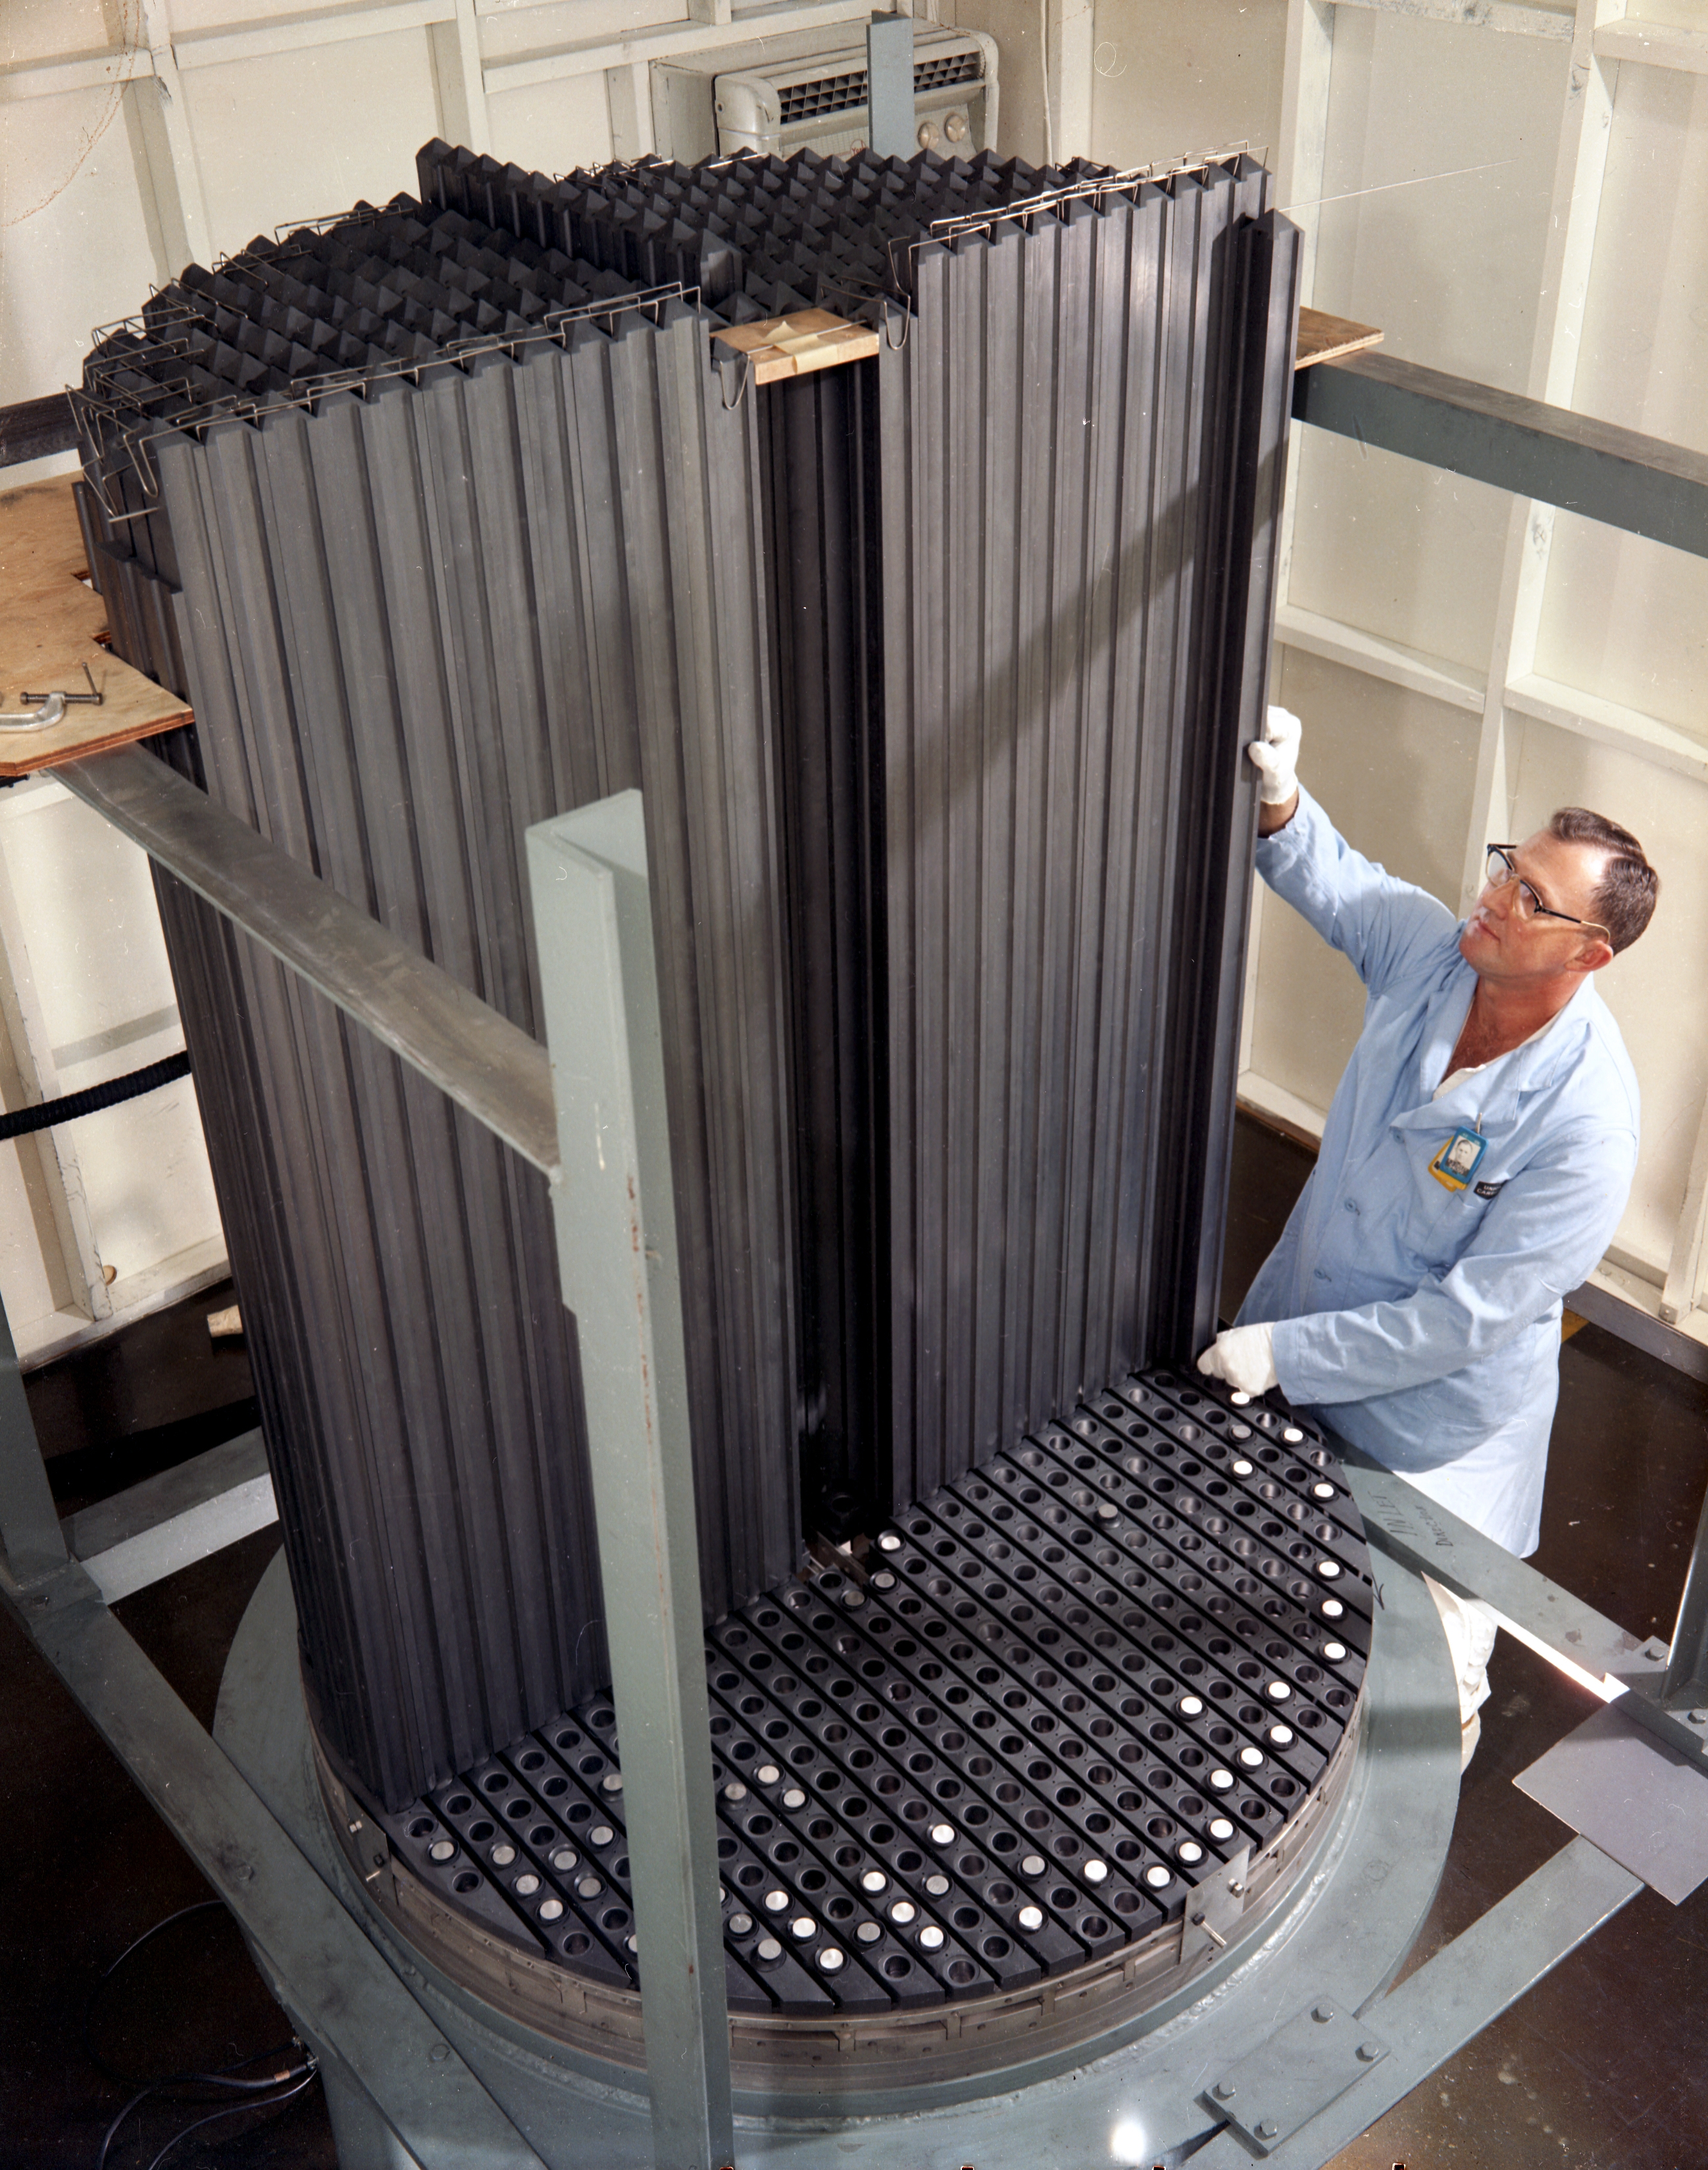
\includegraphics[width=\textwidth]{./images/msre-photo}
      \caption{Graphite assembly for the Molten Salt Reactor Experiment
      \cite{ornl_first-ever_2023}.}
    \end{figure}
    \column{7cm}
    \begin{table}
      \footnotesize
      \centering
      \caption{Thermal-spectrum MSR designs under active development.}
      \begin{tabular}{l l}
        \toprule
        Reactor & Organization \\
        \midrule
        Integral Molten Salt Reactor & Terrestrial Energy \\
        TMSR-LF & CAS (China) \\
        Compact Molten Salt Reactor & Seaborg Technologies \\
        Copenhagen Atomics Waste Burner & Copenhagen Atomics \\
        \bottomrule
      \end{tabular}
    \end{table}
    \begin{table}
      \footnotesize
      \centering
      \caption{Fast-spectrum MSR designs under active development.}
      \begin{tabular}{l l}
        \toprule
        Reactor & Organization \\
        \midrule
        Molten Chloride Fast Reactor & TerraPower \\
        Molten Salt Fast Reactor & CNRS (France) \\
        Stable Salt Reactor - Wasteburner & Moltex Energy \\
        Molten Chloride Salt Fast Reactor & Elysium Industries \\
        \bottomrule
      \end{tabular}
    \end{table}
  \end{columns}
\end{frame}

\begin{frame}[noframenumbering]
  \frametitle{Motivation for MSR Multiphysics Modeling V\&V}
  \textbf{Verification and Validation}

  ``Verification for single-physics codes can be achieved for many applications, but verification
  of multi-physics codes remains a difficult task, especially when the
  coupled problem is solved by iterating different solvers, ...''
  \begin{flushright}
    Tiberga et al. \cite{tiberga_results_2020}
\end{flushright}
  Current V\&V status relating to previous work with Moltres:
  \begin{itemize}
    \item Limited to single-physics verification (e.g., neutronics)
    \item Significant disparities in fidelity between numerical solvers (e.g, Monte Carlo vs
      neutron diffusion)
    \item No validation studies yet, partly due to the lack of MSR experimental data
  \end{itemize}
  \begin{block}{\textbf{Area of Improvement for Moltres for MSR Modeling}}
    \begin{itemize}
      \item Rigorous verification and validation (V\&V) of existing multiphysics capabilities for
        MSR modeling
    \end{itemize}
  \end{block}
\end{frame}

\begin{frame}[noframenumbering]
  \frametitle{V\&V Study 1: Verification of Moltres with the CNRS Benchmark}

  Published in \textit{S.M. Park, M. Munk, "Verification of Moltres for Multiphysics Simulations of
    Fast-Spectrum Molten Salt Reactors," Annals of Nuclear Energy, vol. 173, Aug 2022.}

  \begin{columns}
    \column[t]{6.5cm}
    \begin{block}{\textbf{CNRS Benchmark \cite{tiberga_results_2020}}}
      \begin{itemize}
        \item Consists of three phases
          \begin{itemize}
            \item Phase 0: Single-physics verification
              \begin{itemize}
                \item Step 0.1: Velocity field
                \item Step 0.2: Neutronics
                \item Step 0.3: Temperature
              \end{itemize}
            \item Phase 1: Steady-state coupling
              \begin{itemize}
                \item Step 1.1: Circulating fuel
                \item Step 1.2: Power coupling
                \item Step 1.3: Buoyancy
                \item Step 1.4: Full coupling
              \end{itemize}
            \item Phase 2: Time-dependent coupling
              \begin{itemize}
                \item Step 2.1: Forced convection transient
              \end{itemize}
          \end{itemize}
      \end{itemize}
    \end{block}
    \column[t]{3.5cm}
    \begin{figure}
      \centering
      \includegraphics[width=\columnwidth]{../images/cnrs-geometry}
      \caption{CNRS benchmark problem domain \cite{tiberga_results_2020}}
    \end{figure}
  \end{columns}
\end{frame}

\begin{frame}[noframenumbering]
  \frametitle{V\&V Study 1: Verification of Moltres with the CNRS Benchmark}
  \begin{table}
      \caption{List of software packages and their corresponding model
      specifications for the CNRS Benchmark simulations
      \cite{tiberga_results_2020}.}
      \centering
      \footnotesize
      \begin{tabular}{p{1.8cm} p{3.3cm} p{1.6cm} p{1cm} p{1.1cm}}
          \toprule
          Software & Institute & Numerical method & Mesh & Neutronics model \\
          \midrule
          OpenFOAM & Centre national de la recherche scientifique (CNRS) & Finite volume & 200$\times$200 \newline Non-uniform & $SP_1$ \& $SP_3$ \\
          OpenFOAM & Politecnico di Milano (PoliMi) & Finite volume & 400$\times$400 \newline Uniform & Neutron diffusion \\
          GeN-Foam & Paul Scherrer Institute (PSI) & Finite volume & 200$\times$200 \newline Non-uniform & Neutron diffusion \\
          PHANTOM-$S_N$ DGFlows & Delft University of Technology (TUD) & Discontinuous finite \newline element & 50$\times$50 \newline Uniform & $S_2$ \& $S_6$ \\
          Moltres (This work) & University of Illinois at Urbana-Champaign (UIUC) & Continuous \& discontinuous finite element & 200$\times$200 \newline Uniform & Neutron diffusion \\
          \bottomrule
      \end{tabular}
      \label{table:software}
  \end{table}
\end{frame}

\begin{frame}[noframenumbering]
  \frametitle{V\&V Study 2: MSRE Pump Start-up \& Coast-Down Transients}
  \begin{columns}
    \column[t]{4cm}
    \begin{figure}
      \centering
      \includegraphics[width=.9\columnwidth]{../images/msre-transient}
      \caption{Control rod response to fuel pump start-up and coast-down
      \cite{prince_zero-power_1968}.}
    \end{figure}
    \hfill
    \column[t]{4cm}
    \begin{figure}
      \centering
      \includegraphics[width=.9\columnwidth]{../images/msre-rod-worth}
      \caption{Integral rod worth \cite{prince_zero-power_1968}.}
    \end{figure}
    \hfill
    \column[t]{4cm}
    \begin{figure}
      \centering
      \includegraphics[width=.9\columnwidth]{images/msre-2d}
      \caption{2-D axisymmetric model of the MSRE with fuel (gray) and graphite (white) regions.}
    \end{figure}
  \end{columns}
\end{frame}

\begin{frame}[noframenumbering]
  \frametitle{Turbulence Models}
  Numerous types of turbulence models exist at various levels of fidelity. From lowest to highest
  computational complexity:
  \begin{itemize}
      \item RANS-based models
      \begin{itemize}
          \item Eddy viscosity models
          \begin{itemize}
              \item Algebraic models
              \item One-equation
              \item Two-equation models
          \end{itemize}
          \item \gls{RSM}
      \end{itemize}
      \item \gls{DES}
      \item \gls{LES}
      \item \gls{DNS}
  \end{itemize}
\end{frame}

\begin{frame}[noframenumbering]
  \frametitle{Turbulence Models}
  \gls{RANS}-based models are based on the RANS equations obtained by applying time-averaging on
  the fluid flow equations:
  \begin{gather}
      \frac{\partial U_i}{\partial t} + U_j \frac{\partial u_i}{\partial x_j} =
      -\frac{1}{\rho} \frac{\partial P}{\partial x_i} + \nu \nabla^2 U_i -
      \frac{\partial \langle u_i u_j \rangle}{x_j}
      \shortintertext{where}
      U = \mbox{ mean component,} \qquad u = \mbox{ fluctuating component.} \nonumber
  \end{gather}
  Eddy viscosity models operate on the eddy viscosity hypothesis:
  \begin{align}
      \langle u_iu_j \rangle =& \frac{2}{3}k \delta_{ij} - \nu_T \left(
      \frac{\partial U_i}{\partial x_j} + \frac{\partial U_j}{\partial x_i}
      \right)
      \shortintertext{where}
        \nu_T =& \mbox{ eddy viscosity.} \nonumber
  \end{align}
  The various eddy viscosity models mainly differ in their approach to the closure problem of
  calculating the eddy viscosity.
\end{frame}

\begin{frame}[noframenumbering]
  \frametitle{Control Rods in MSRs}
  \begin{table}
    \centering
    \footnotesize
    \caption{List of MSR designs which contain control rods.}
    \begin{tabular}{l l}
      \toprule
      Reactor & Spectrum \\
      \midrule
      Molten Salt Reactor Experiment & Thermal \\
      Integral Molten Salt Reactor & Thermal \\
      TMSR-LF1 & Thermal \\
      Liquid Fluoride Thorium Reactor & Thermal \\
      Compact Molten Salt Reactor* & Thermal \\
      Stable Salt Reactor - Wasteburner* & Fast \\
      ThorCon Reactor* & Thermal \\
      \bottomrule
    \end{tabular}
  \end{table}
  Asterisks indicate MSR designs with ``control'' rods labeled as ``shutdown'' rods.
\end{frame}

\begin{frame}[noframenumbering]
  \frametitle{Hybrid $S_N$-Diffusion Method: Literature Review}
  \textbf{Absorber Blackness} \\
  Encompasses a broad class of procedures for generating boundary conditions to match approximate
  solutions of low-order methods to more accurate solutions of high-order methods
  \cite{davison_influence_1951, spinks_extrapolation_1965, pellaud_extrapolation_1968,
  mendelson_two-dimensional_1969}. \\
  The boundary conditions are generalizations of the Marshak boundary condition, which in 1-D are
  of the form:
  %
  \begin{align}
    \frac{\phi(x)}{d\phi(x)/dx} =& \lambda \label{eq:marshak}
    \shortintertext{where}
    \phi =& \mbox{ neutron scalar flux,} \nonumber \\
    \lambda =& \mbox{ linear extrapolation length.} \nonumber
  \end{align}
  %
  Alternatively, the internal boundary conditions may be replaced with ``effective'' diffusion
  coefficients and absorption cross sections \cite{bretscher_computing_1997}.
\end{frame}

\begin{frame}[noframenumbering]
  \frametitle{Hybrid $S_N$-Diffusion Method: Literature Review}
  \textbf{Method of Equivalent Cross Sections (MECS)}
  \begin{columns}
    \column[t]{7cm}
    Implemented in the CITATION nodal diffusion code for control rod modeling in High-Temperature
    Gas-Cooled Reactors (HTGR). \\
    \textbf{Methodology}
    \begin{enumerate}
      \item Run a high-fidelity 1-D neutron transport calculation on a representative supercell of
        the control rod and its vicinity
      \item Match the net leakage rates from the transport solver to the diffusion solver using an
        analytic formula
      \item Solve for the equivalent diffusion coefficients
    \end{enumerate}
    \textbf{Limitations}
    \begin{enumerate}
      \item The solving procedure places geometric constraints on the geometry nodalization
      \item Incompatible with reactor geometries which contain control rods that are too close
      \item Only applicable for coarse-mesh diffusion solvers
    \end{enumerate}
    \column[t]{4cm}
    \begin{figure}
      \centering
      \includegraphics[width=.75\columnwidth]{../images/mecs-geometry}
      \caption{Geometry of the supercell (top) and the diffusion solver mesh (bottom)
        \cite{fen_modelling_1992}.}
    \end{figure}
  \end{columns}
\end{frame}

\begin{frame}[noframenumbering]
  \frametitle{Hybrid $S_N$-Diffusion Method: Literature Review}
  \textbf{Response-Based Methods}
  \vspace{.3cm}

  Another technique applied to modeling control rods in HTGRs with nodal diffusion codes. \\
  Uses neutron transport solutions to generate response functions, which relate flux-based
  quantities (e.g., incident partial currents $\Rightarrow$ average nodal flux and outgoing partial
  currents)
  \vspace{.3cm}

  \textbf{Examples}
  \begin{enumerate}
    \item Fen et al. \cite{fen_modelling_1992} developed the Response Matrix Method which generates
      boundary conditions from response functions.
    \item Rahnema et al. \cite{rahnema_advanced_2011} developed the integrated diffusion/transport
      (IDT) method which generates coupling coefficients used in nodal diffusion calculations.
  \end{enumerate}
\end{frame}

\begin{frame}[noframenumbering]
  \frametitle{Hybrid $S_N$-Diffusion Method: Preliminary Results}
  \textbf{Differences in Neutron Multiplication Factor, $k$}
  \begin{columns}
    \column{12cm}
  \begin{table}[htb!]
    \centering
    \scriptsize
    \caption{Differences in $k$ estimates for Cases 1a, 1b, 2a, 2b, 3a, and 3b for the $S_8$ neutron
      transport, neutron diffusion, and Hybrid $S_N$-Diffusion methods relative to OpenMC-MG.}
    \begin{tabular}{c S[table-format=+1.5(2)] S[table-format=+1.5(2)] S[table-format=+1.5(2)]
        S[table-format=+1.5(2)] S[table-format=+1.5(2)] S[table-format=+1.5(2)]}
      \toprule
      \multirow{2}{*}{\textbf{Method}} & \multicolumn{6}{c}{$\bm{k-k_{MG}}$} \\
      \cmidrule{2-7}
      & {\textbf{Case 1a}} & {\textbf{Case 1b}} & {\textbf{Case 2a}} &
      {\textbf{Case 2b}} & {\textbf{Case 3a}} & {\textbf{Case 3b}} \\
      \midrule
      $S_8$     & +0.00020(33) & -0.00036(54) & +0.00026(66) & -0.00069(50) & -0.00008(48) & -0.00078(50) \\
      Diffusion & +0.00021(33) & -0.00172(54) & -0.00861(66) & -0.01265(50) & -0.00912(48) & -0.01280(50) \\
      Hybrid    & {N/A}        & {N/A}        & +0.00060(66) & -0.00152(50) & +0.00028(48) & -0.00162(50) \\
      \bottomrule
    \end{tabular}
    \label{table:ckdiff1}
  \end{table}
  %
  \begin{table}[htb!]
    \centering
    \scriptsize
    \caption{Differences in $k$ estimates for Cases 4a, 4b, 5a, and 5b for the $S_8$ neutron
      transport, neutron diffusion, and Hybrid $S_N$-Diffusion methods relative to OpenMC-MG.}
    \begin{tabular}{c S[table-format=+1.5(2)] S[table-format=+1.5(2)] S[table-format=+1.5(2)]
      S[table-format=+1.5(2)]}
      \toprule
      \multirow{2}{*}{\textbf{Method}} & \multicolumn{4}{c}{$\bm{k-k_{MG}}$} \\
      \cmidrule{2-5}
      & {\textbf{Case 4a}} & {\textbf{Case 4b}} & {\textbf{Case 5a}} &
      {\textbf{Case 5b}} \\
      \midrule
      $S_8$     & +0.00021(37) & +0.00006(63) & -0.00017(50) & -0.00027(53) \\
      Diffusion & +0.00000(37) & +0.00073(63) & -0.00872(50) & +0.00277(53) \\
      Hybrid    & {N/A}        & {N/A}        & +0.00070(50) & {N/A}    \\
      \bottomrule
    \end{tabular}
    \label{table:ckdiff2}
  \end{table}
  %
\end{columns}
\end{frame}

%\begin{frame}[noframenumbering]
%  \frametitle{Hybrid $S_N$-Diffusion Method: Proposed Work}
%  \textbf{Investigate and rectify potential rod cusping errors}
%  \vspace{.2cm}
%  \begin{columns}
%    \column[t]{6.5cm}
%    Rod cusping occurs when the control rod boundary does not align perfectly with the mesh element
%    boundaries when modeling time-dependent control rod insertion/withdrawal.
%    \vspace{.1cm}
%  
%    Potential solutions:
%    \begin{itemize}
%      \item Adaptive meshing
%      \item Approximate flux-volume weighting of cross sections
%      \item Projection-based cusping treatment \cite{schunert_control_2019}
%      \begin{itemize}
%        \item Projection of piecewise constant cross sections onto a set of Legendre polynomials
%        \item Exact integration of the FEM weak form is achieved
%      \end{itemize}
%    \end{itemize}
%    \column[t]{5.5cm}
%    \begin{figure}
%      \centering
%      \includegraphics[width=.65\columnwidth]{images/cusping}
%      \caption{Illustration of control rod cusping effect.}
%      \includegraphics[width=.65\columnwidth]{images/control-drum}
%      \caption{Adaptive meshing of a rotating control drum.}
%    \end{figure}
%  \end{columns}
%\end{frame}

